\clearpage%
%\ifodd\value{page}\hbox{}\newpage\fi%
\unlessboolexpr{test{\ifnumequal{\intcalcMod{\value{page}}{4}}{2}}}{%
	\section*{Notes / Dessins / Poésies}\hbox{}
	\def\width{16}
	\def\hauteur{20}
	\begin{center}
		
\begin{tikzpicture}[x=1cm, y=1cm, semitransparent]
		\draw[step=4mm, line width=0.1mm, blue!50!white] (0,0) grid (\width,\hauteur);
		\end{tikzpicture}
	\end{center}
	\newpage}
%\cleardoublepage
\thispagestyle{empty}%
{\centering
\vspace*{15mm}

\includegraphics[width=.90\textwidth]{fig/bowling0.pdf}
\vspace*{25mm}


\includegraphics[width=.90\textwidth]{fig/bowling1.pdf}
\par
}

\clearpage

\begin{center}
{\Huge Plusieurs activités sont financées par la}
\vspace*{5mm}
\par

\includegraphics[width=0.85\textwidth]{fig/regie_fribourg.pdf}
\end{center}

\vfill
\begin{center}
	{\Huge et}
\end{center}
\vfill

\begin{center}
{\Huge par les comités de la Saint Nicolas\vspace*{1mm}\\
du Collège St-Michel}
\vspace*{5mm}
\par

\includegraphics[width=0.8\textwidth]{fig/csm.jpg}
\end{center}


\clearpage
\thispagestyle{empty}%
{\centering
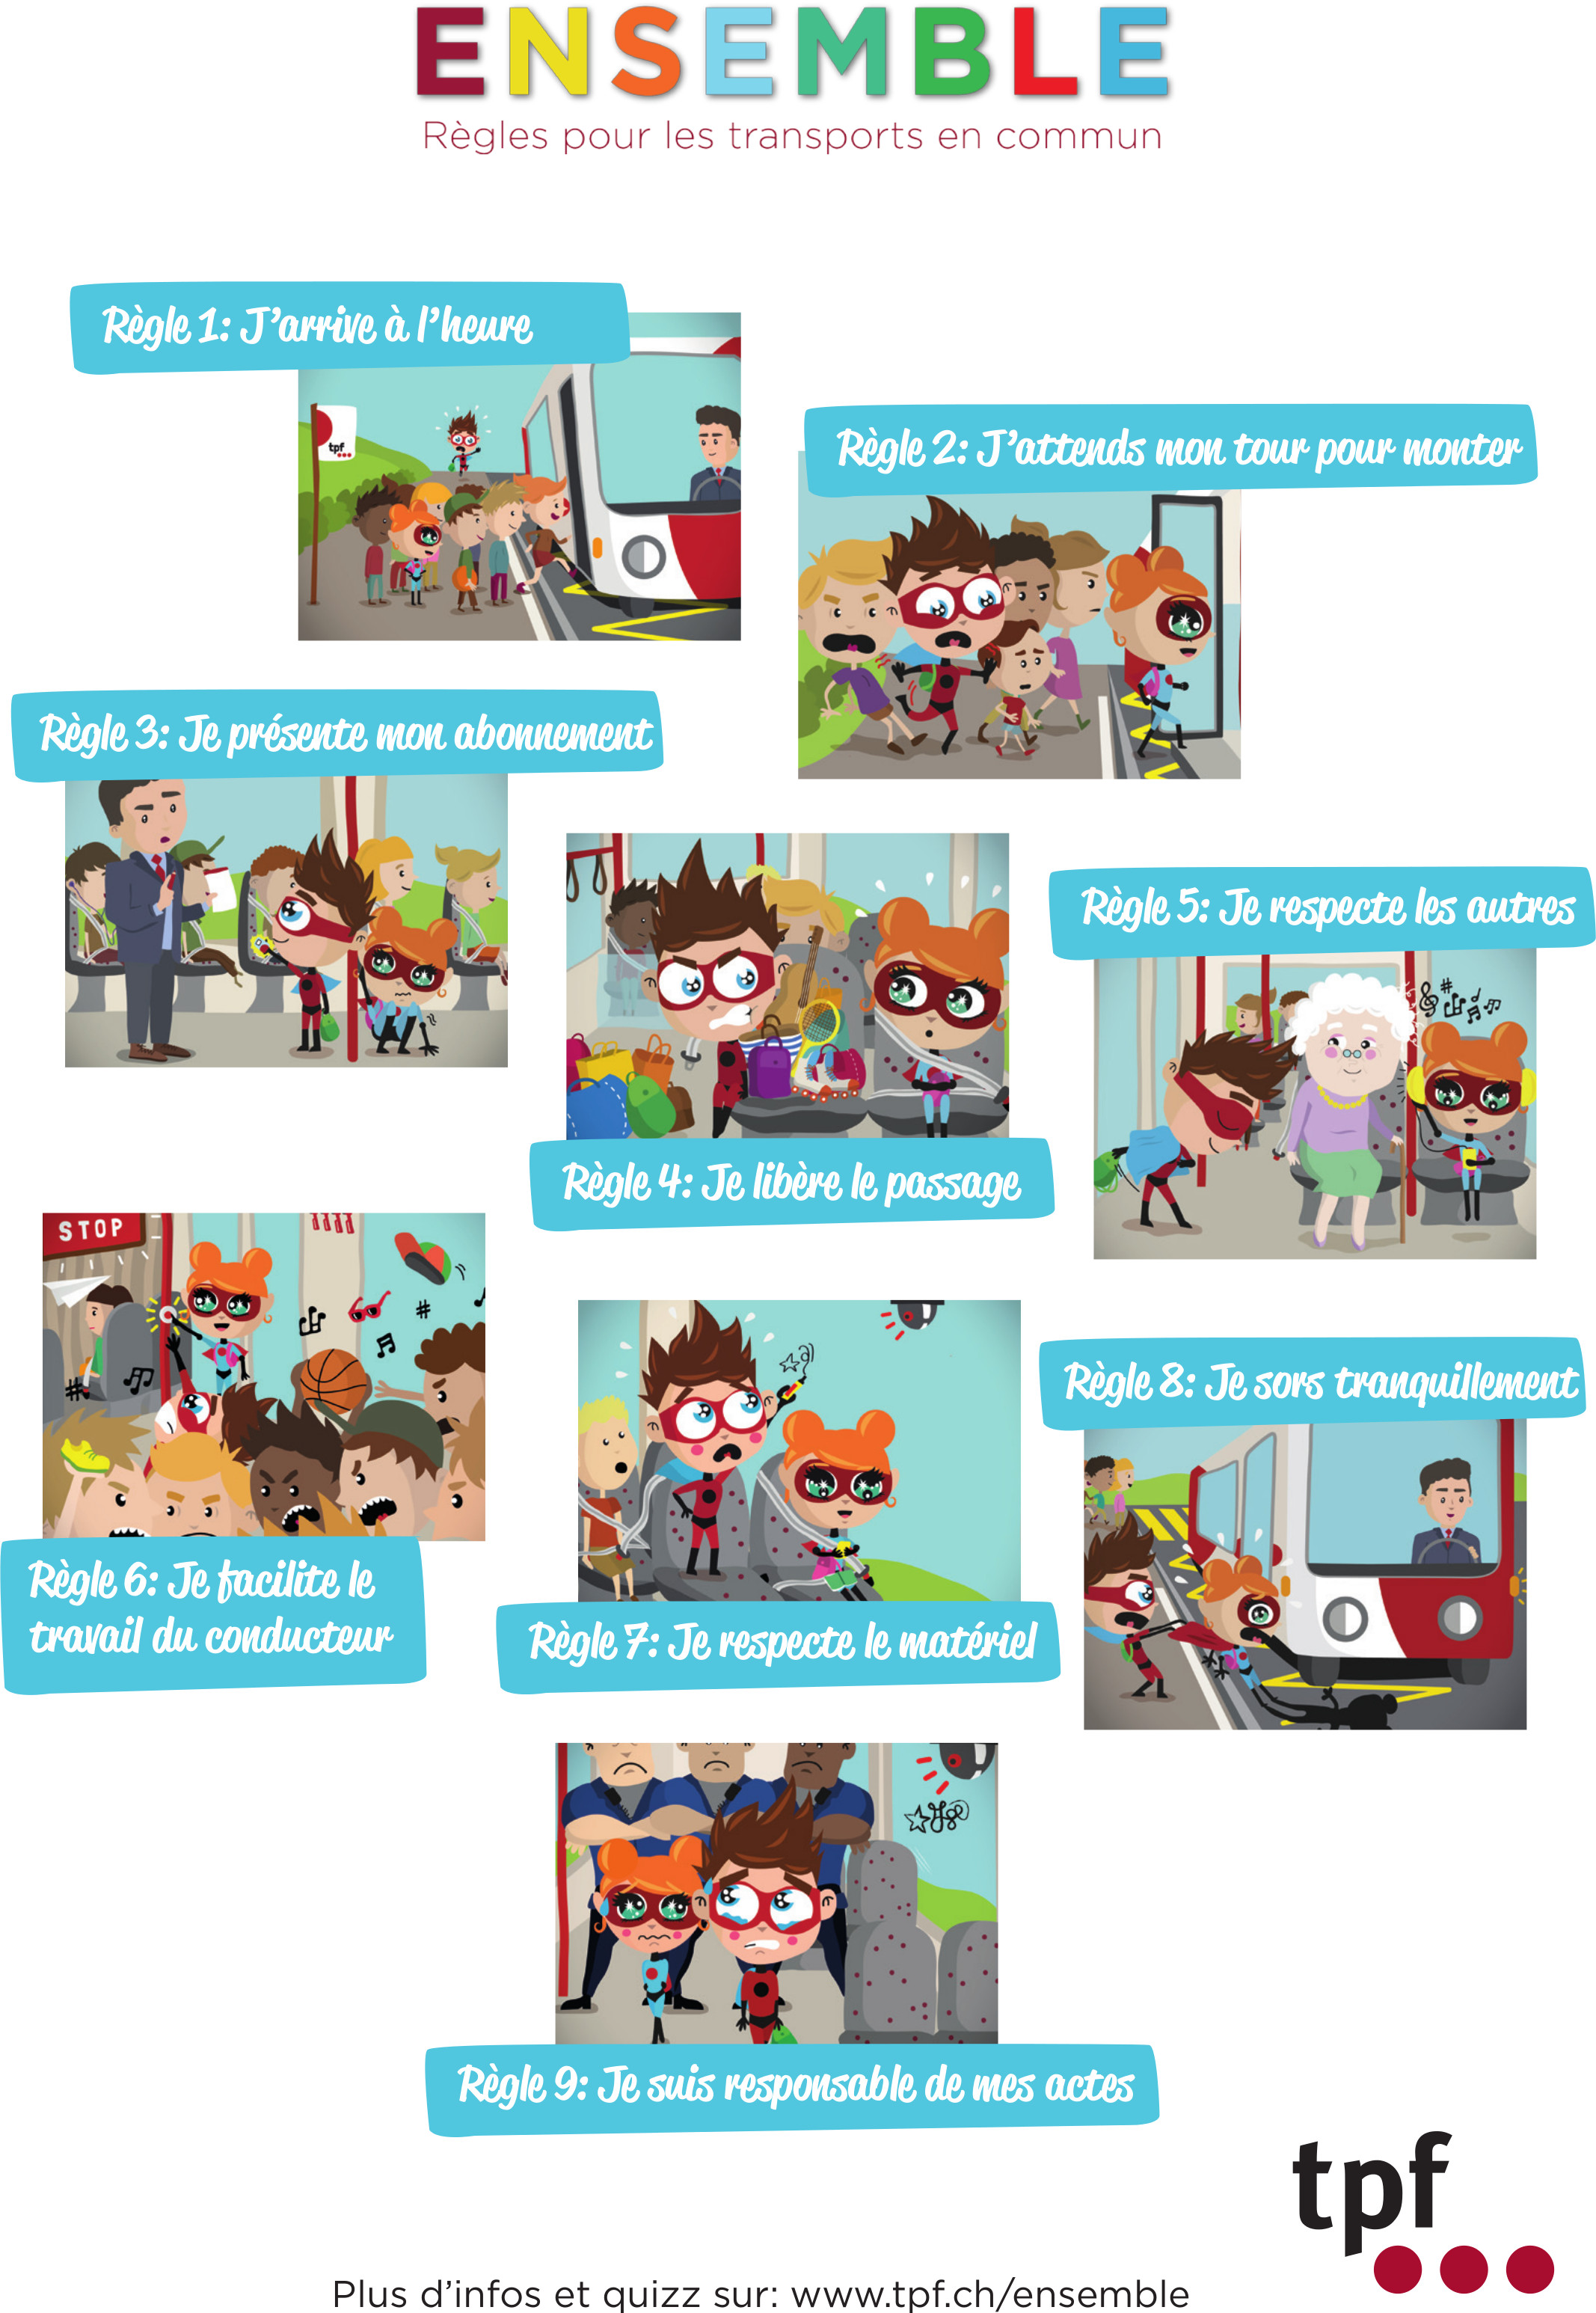
\includegraphics[width=.96\textwidth]{fig/ensemble.jpg}
\par
}
\clearpage
\section*{Réseau régional\\Stadtnetz Regio}
\begin{textblock}{2}(11,1.3)

\includegraphics[width=3cm]{fig/tpf.pdf}
\end{textblock}
\begin{center}
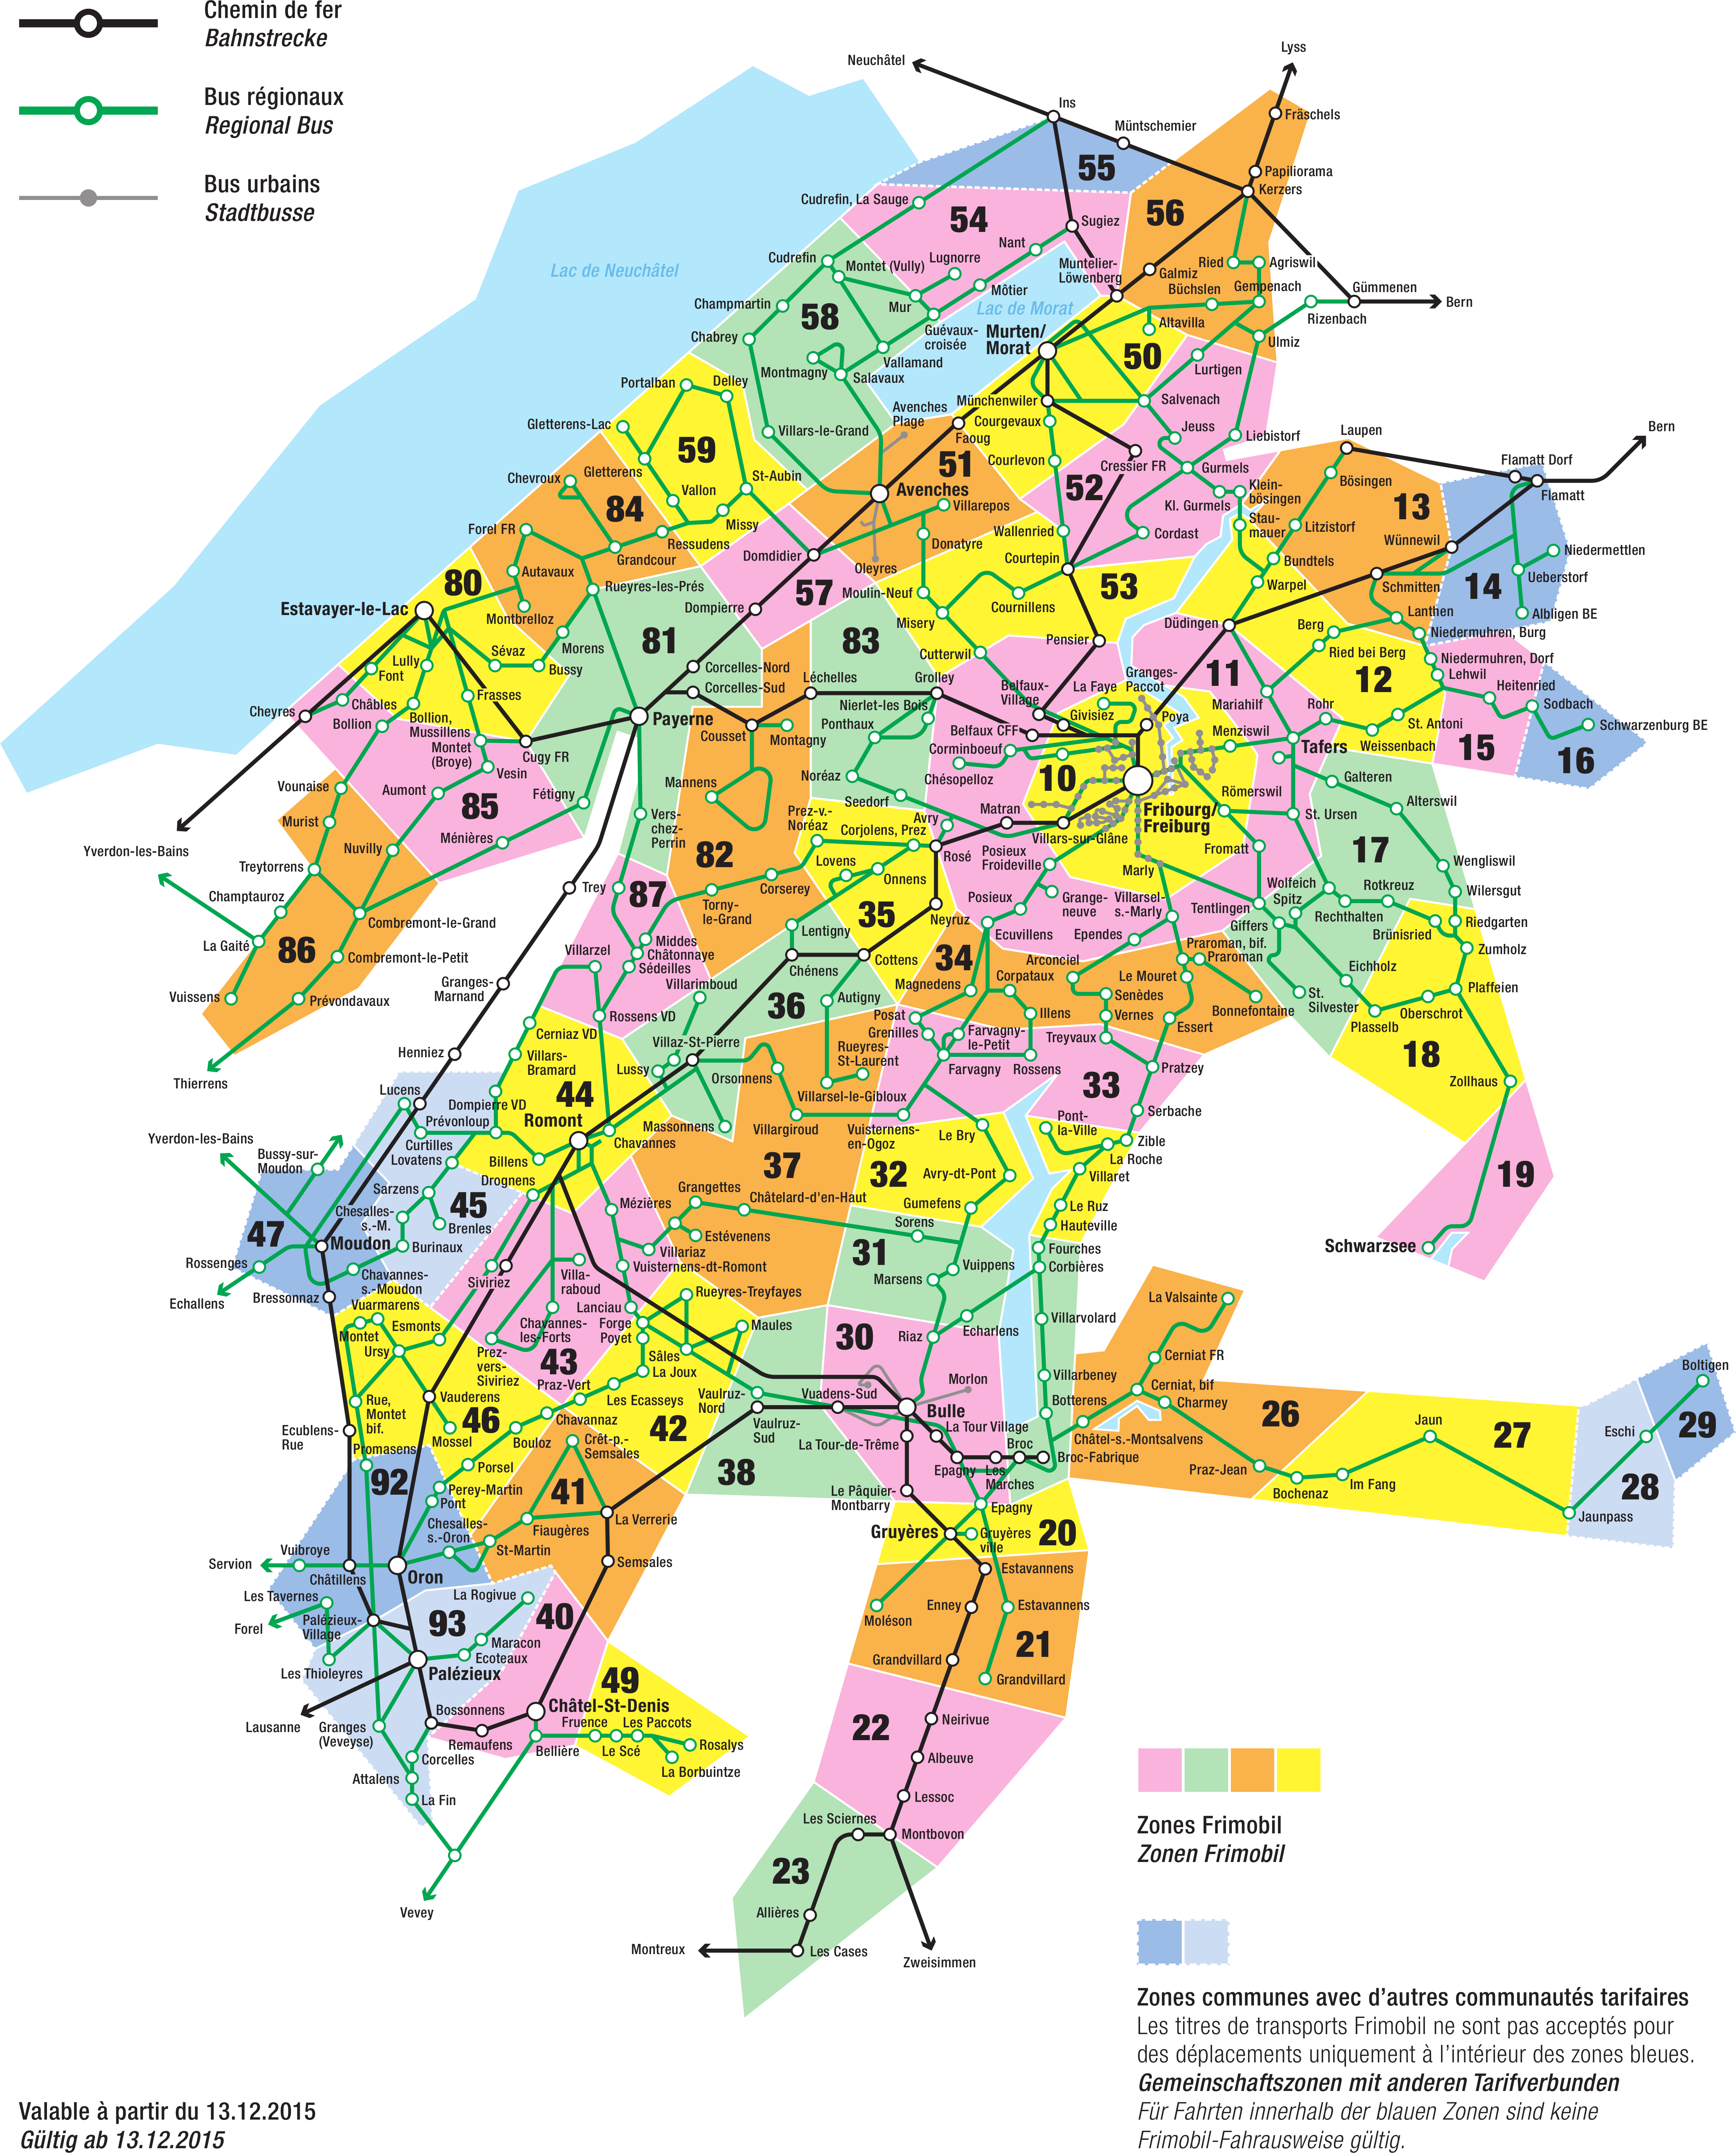
\includegraphics[width=\textwidth]{fig/plan_regional.png}
\end{center}
\clearpage%
\thispagestyle{empty}%
\section*{Réseau Agglo Fribourg\\Stadtnetz Freiburg}%
\begin{textblock}{2}(11,1.3)%

\includegraphics[width=3cm]{fig/tpf.pdf}%
\end{textblock}%
\begin{center}
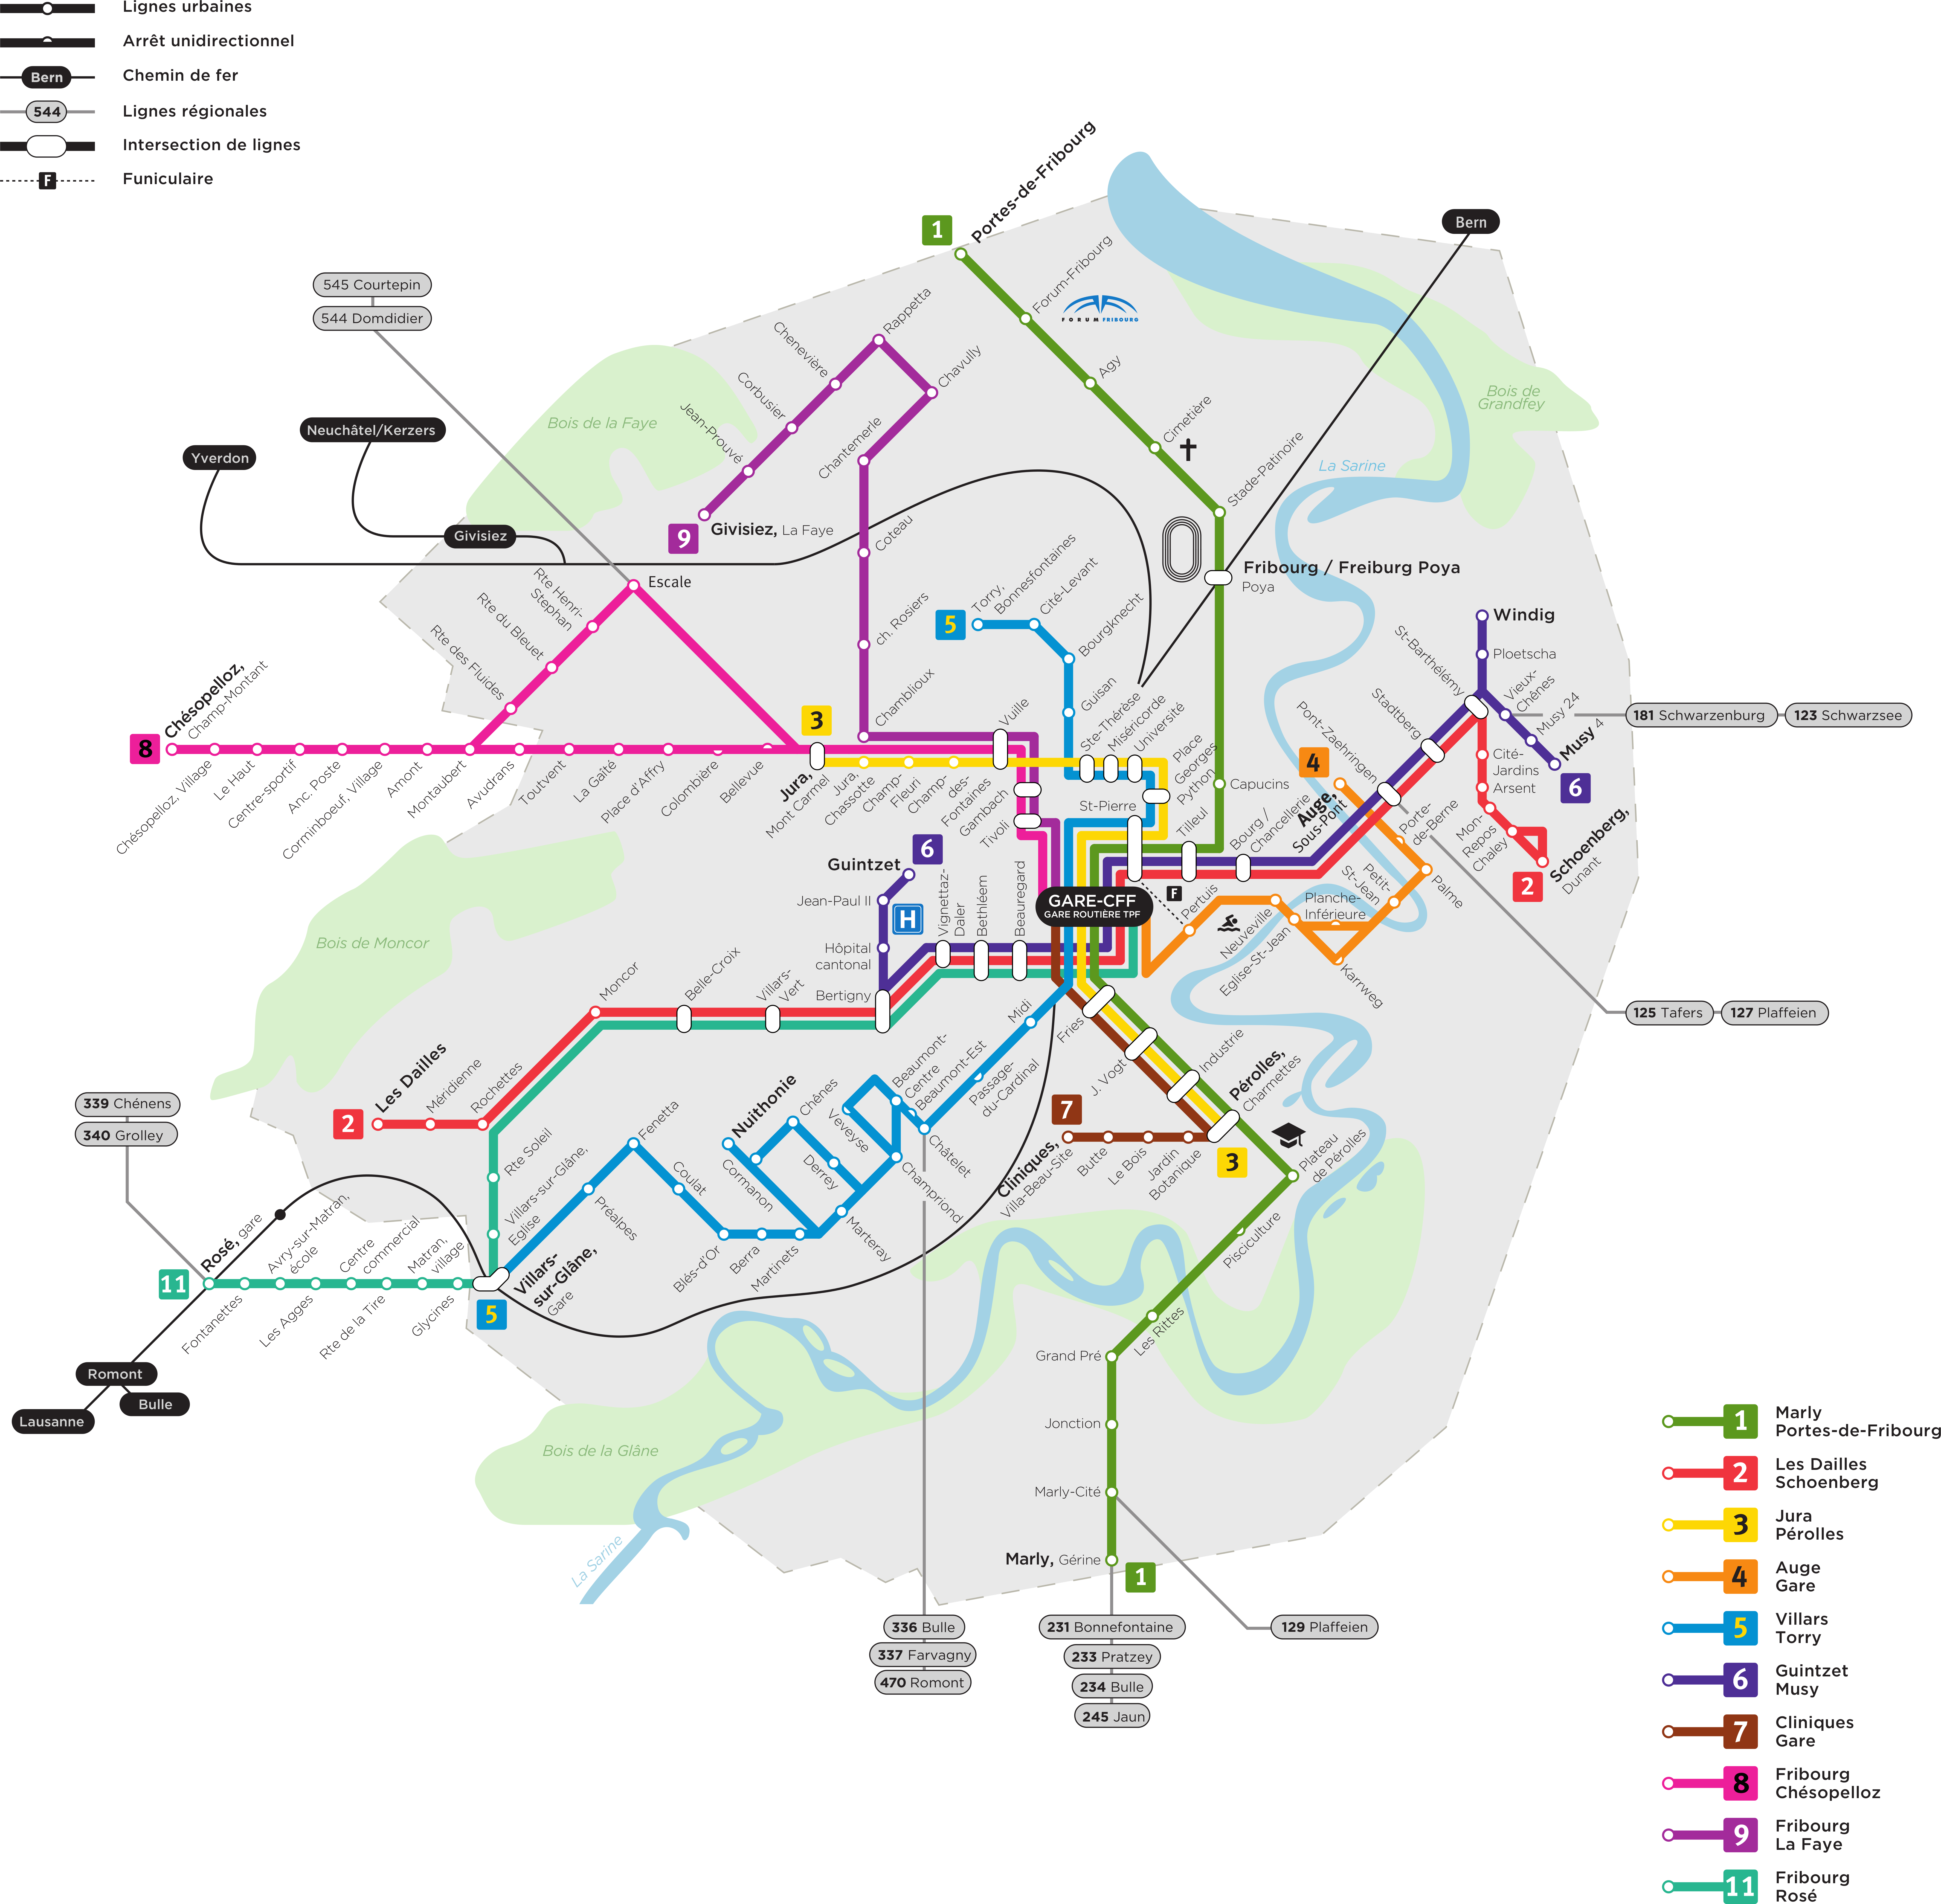
\includegraphics[width=\textwidth]{fig/plan_zone_10.png}
\end{center}
